\documentclass[12pt,a4paper,oneside]{article}
\usepackage{graphicx,setspace,float,fancyhdr,listings,xcolor,placeins,xeCJK,tocloft,enumerate,amsmath}
\usepackage[dvipsnames]{xcolor}
\renewcommand{\cftsecleader}{\cftdotfill{\cftdotsep}} % Enable dot leaders in TOC
\renewcommand{\cftdotsep}{1} % Adjust dot spacing

\date{\Large 2024.11.21}
\author{陈海弘}

\setCJKmainfont[AutoFakeBold=3]{STFangsong} % CJK Font Setup
\setcounter{tocdepth}{3} % Set TOC depth
\setstretch{1.25} % Line spacing

% Page header and footer setup
\setlength{\headheight}{13.6pt}
\addtolength{\topmargin}{-1.6pt}
\pagestyle{fancy}
\fancyhf{}
\fancyhead[C]{\small Machine Learning} % Center header
\fancyfoot[C]{\small \thepage} % Center footer

% Code highlighting setup
\lstset{
    language=Python,
    basicstyle=\ttfamily\small,
    keywordstyle=\bfseries\color{NavyBlue},
    commentstyle=\itshape\color{red!50!green!50!blue!50},
    stringstyle=\bfseries\color{PineGreen!90!black},
    emph={self}, 
    emphstyle=\bfseries\color{Rhodamine},
    backgroundcolor=\color{black!3},
    frame=shadowbox,
    frameround=fttt,
    numbers=left,
    numberstyle=\tiny,
    stepnumber=1,
    numbersep=5pt,
    breaklines=true,
    columns=flexible,
    xleftmargin=1em,
    xrightmargin=-2em,
    aboveskip=1em,
    framexleftmargin=2em,
    escapeinside=``,
}

% Title setup
\title{
    \vspace*{-2cm}
    
\includegraphics[width=0.8\textwidth]{SYSULogo.pdf} \\[1em]
    \vfill
    \LARGE \textbf{机器学习实验报告4} \\[1em]
    \Large
    \begin{tabular}{rl}
        \textbf{姓名:} & \textbf{陈海弘} \\
        \textbf{学号:} & \textbf{23354049}
    \end{tabular}
    \vfill
}

\begin{document}
\maketitle
\newpage
\tableofcontents
\newpage

\section{摘要}
\qquad 本次实验是关于红酒品质的预测,使用的是一个关于红酒品质的数据集,总共有1599个样本,每个样本包含11个特征以及1个标签,每个标签的取值是连续的。本次实验已经按照8:2的比例划分成了训练数据集'wine\_train.csv'以及测试数据集'wine\_test.csv',且每个数据集都已经做了归一化处理。

引用的库有pandas、torch、matplotlib、numpy等,其中最重要的是torch库,因为本次实验是关于神经网络的搭建和训练的。本次试验用的pytorch版本是2.5.1。

Tensor和ndarray相似,但是Tensor可以利用GPU加速。
\section{神经网络中的前向传播和后向传播}
\subsection{实验要求}
\qquad Red Wine Quality是一个关于红酒品质的数据集,总共有1599个样本,每个样本包含11个(都是连续的)特征以及1个标签,每个标签的取值是连续的。本次实验已经按照8:2的比例划分成了训练数据集'wine\_train.csv'以及测试数据集'wine\_test.csv',且每个数据集都已经做了归一化处理。

\subsection{数据读取}
\qquad 读入训练数据集'wine\_train.csv'与测试数据集'wine\_test.csv'。

\begin{lstlisting}
    train_data = pd.read_csv('wine_train.csv')
    test_data = pd.read_csv('wine_test.csv')
\end{lstlisting}

\subsection{神经网络搭建}
\qquad 利用线性层和激活函数搭建一个神经网络,要求输入和输出维度与数据集维度一致,而神经网络深度、隐藏层大小、激活函数种类等超参数自行调整。

输入维度为11,输出维度为1,所以输入层到隐藏层、隐藏层到隐藏层、隐藏层到输出层的维度分别为11、128、32。

神经网络深度是3层,所以定义一个神经网络类WineNet,继承自nn.Module。在构造函数中定义了三个全连接层,分别是输入层到隐藏层、隐藏层到隐藏层、隐藏层到输出层。

激活函数是ReLU函数,即$ReLU(x) = max(0, x)$。还有其他的激活函数,例如sigmoid函数,即$sigmoid(x) = \frac{1}{1 + e^{-x}}$,以及tanh函数,即$tanh(x) = \frac{e^x - e^{-x}}{e^x + e^{-x}}$。

在forward函数中定义了神经网络的前向传播过程,即将输入数据经过全连接层和激活函数处理后输出。

\begin{lstlisting}
    class WineNet(nn.Module):
    def __init__(self):
        super (WineNet, self).__init__()
        self.fc1 = nn.Linear(11,128)
        self.fc2 = nn.Linear(128,32)
        self.fc3 = nn.Linear(32,1)
    def forward(self,x):
        x = F.relu(self.fc1(x))
        x = F.relu(self.fc2(x))
        x = self.fc3(x)
        return x
net = WineNet()
print(net)
\end{lstlisting}

\begin{figure}[H]
    \centering
    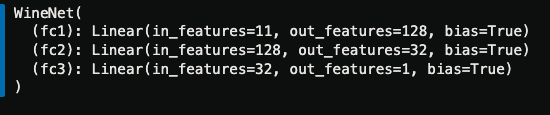
\includegraphics[width=0.8\textwidth]{image/1.png}
    \caption{神经网络结构}
\end{figure}

\subsection{训练}
\qquad 用梯度下降法进行模型参数更新,记下每轮迭代中的训练损失和测试损失。

\begin{itemize}
    \item \textbf{数据准备}:将 pandas 数据转换为 PyTorch 张量,特征数据 $X$ 选取除最后一列外的所有列,标签数据 $y$ 选取最后一列,并 reshape 为 $(1, -1)$。
    \item \textbf{训练阶段}:初始化神经网络模型,使用均方误差 (MSE) 作为损失函数,使用随机梯度下降 (SGD) 优化器,学习率为 $0.01$,迭代次数为 $100$ 次。
    \item \textbf{循环过程}:
    \begin{itemize}
        \item 将模型设置为训练模式。
        \item 进行前向传播,计算训练损失。
        \item 反向传播并更新模型参数。
        \item 注意清空梯度,避免梯度累积导致性能下降。
    \end{itemize}
    \item \textbf{测试阶段}:将模型设置为测试模式,进行前向传播并计算测试损失。
\end{itemize}

\begin{lstlisting}
X_train = torch.tensor(train_data.iloc[:, :-1].values, dtype=torch.float32)  # 训练特征
y_train = torch.tensor(train_data.iloc[:, -1].values, dtype=torch.float32).view(-1, 1)  # 训练标签
X_test = torch.tensor(test_data.iloc[:, :-1].values, dtype=torch.float32)  # 测试特征
y_test = torch.tensor(test_data.iloc[:, -1].values, dtype=torch.float32).view(-1, 1)  # 测试标签

net = WineNet()# 初始化模型
criterion = nn.MSELoss()# 定义损失函数

learning_rate = 0.01
epochs = 100

train_losses = []
test_losses = []

optimizer = torch.optim.SGD(net.parameters(),lr = learning_rate)

for epoch in range(epochs):
    net.train()# 训练阶段
    output = net(X_train)# 前向传播
    train_loss = criterion(output, y_train)  # 计算训练损失

    optimizer.zero_grad()
    train_loss.backward()
    optimizer.step()

    net.zero_grad()# 清空梯度

    # 测试阶段
    net.eval()  # 设置为评估模式
    with torch.no_grad():  # 禁用梯度计算
        test_output = net(X_test)  # 前向传播
        test_loss = criterion(test_output, y_test)  # 计算测试损失

    # 记录每轮的训练损失和测试损失
    train_losses.append(train_loss.item())
    test_losses.append(test_loss.item())

    if epoch % 10 == 0:
        print(f'Epoch[{epoch+1}/{epochs}],TrainLoss:{train_loss.item():.4f},TestLoss:{test_loss.item():.4f}')
\end{lstlisting}

\begin{figure}[H]
    \centering
    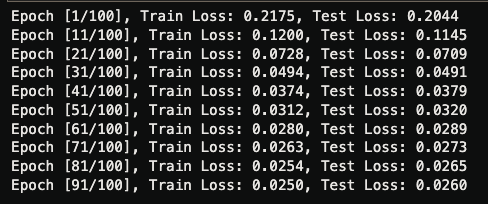
\includegraphics[width=0.8\textwidth]{image/2.png}
    \caption{训练损失和测试损失}
\end{figure}

可以看到,训练损失和测试损失都随着迭代次数的增加而减小,说明模型在逐渐收敛。

除了用PyTorch的优化器来更新net中的参数外,还可以手动更新参数,用梯度下降法手动实现。
\begin{lstlisting}
    with torch.no_grad():  # 禁用梯度计算
    for f in net.parameters():
        f.data.sub_(f.grad.data * learning_rate)  # 手动梯度下降更新参数

\end{lstlisting}


\subsection{训练损失测试损失展示}

\begin{lstlisting}
    plt.plot(range(len(train_losses)), train_losses, label='Train Loss')
plt.plot(range(len(test_losses)), test_losses, label='Test Loss')
plt.xlabel('Epochs')
plt.ylabel('Loss')
plt.title('Training and Testing Loss')
plt.legend()
plt.grid()
plt.show()
\end{lstlisting}

\begin{figure}[H]
    \centering
    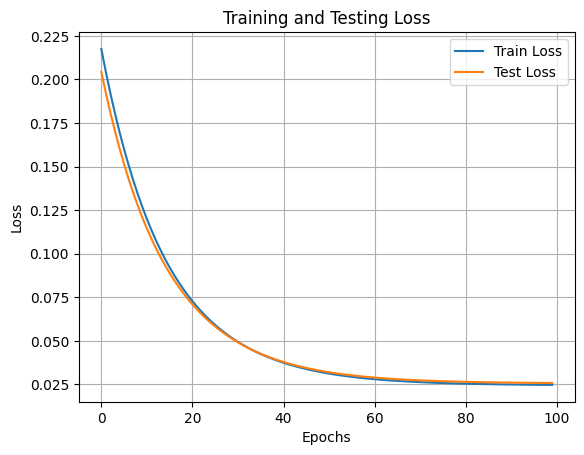
\includegraphics[width=0.8\textwidth]{image/3.png}
    \caption{训练损失和测试损失}
\end{figure}

该图显示了训练损失和测试损失随迭代次数的变化情况。可以看到,训练损失和测试损失都随着迭代次数的增加而减小,说明模型在逐渐收敛。并且训练损失和测试损失的差距在逐渐减小,说明模型在逐渐泛化。
\section{总结}
\qquad 这次试验首先学习了pytorch库,还有tensor的创建,运算,和ndarray的转换。然后学习了神经网络的搭建,前向传播和后向传播。最后学习了如何用pytorch训练一个神经网络。

实验主要围绕对红酒品质的预测,用神经网络来预测红酒的品质。我认为我需要注意的地方有,在神经网络的搭建的时候,要注意输入和输出的维度,以及神经网络的深度和隐藏层的大小。在训练的时候,要注意梯度的清空,避免梯度累积导致性能下降。
\end{document}
